\section{Power Routing.}
\label{section::powerrouting}


\PowerRouting relies on two central concepts.  First, it exploits \emph{shuffled topologies} for power distribution to increase the connectivity between servers and diverse PDUs.  Shuffled topologies spread responsibility to sustain the load on a failing PDU, reducing the required reserve capacity per PDU.  Second, \PowerRouting relies on a \emph{scheduling} algorithm to assign servers' load across redundant distribution paths while balancing loads over PDUs and AC phases.  When loads are balanced, the provisioned capacity of major power infrastructure components (PDUs, UPSs, generators, and utility feeds) can be reduced, saving capital costs.  We first detail the design and advantages of shuffled topologies, and then discuss \PowerRouting.

\subsection{Shuffled Topologies.}
\label{section::intermixed}

\begin{figure*}[t]
\centering
\subfigure[Wrapped (conventional)]{
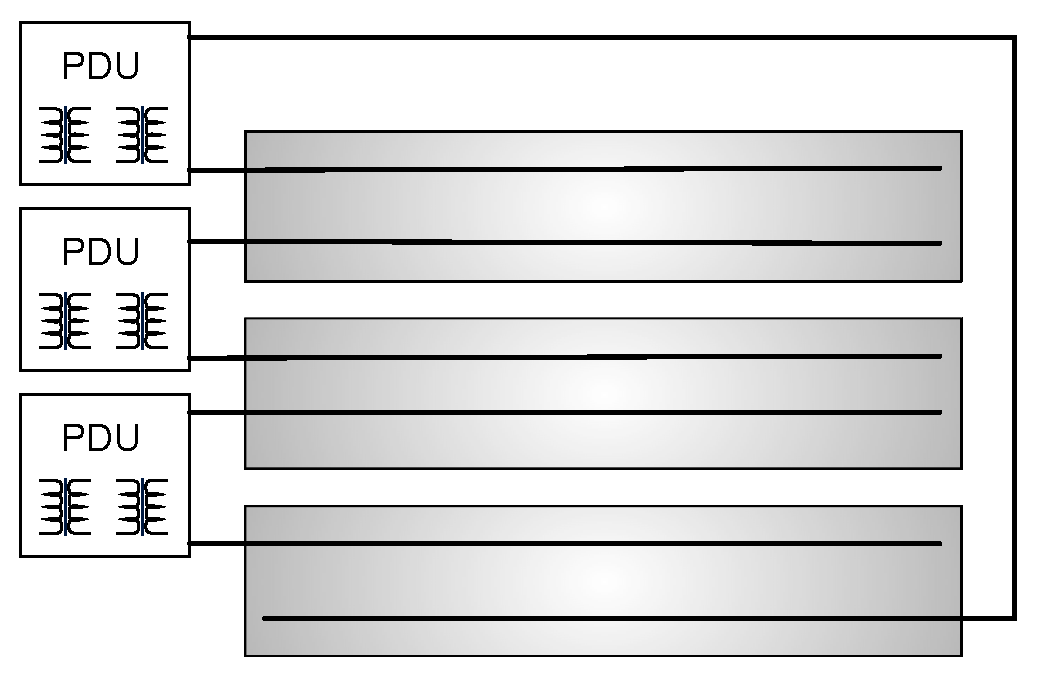
\includegraphics[scale=.3]{Appendices/PowerRouting/figure/standard3.eps}
\label{figure::wrapped}
}
\hspace{0.3in}
\subfigure[Fully-connected]{
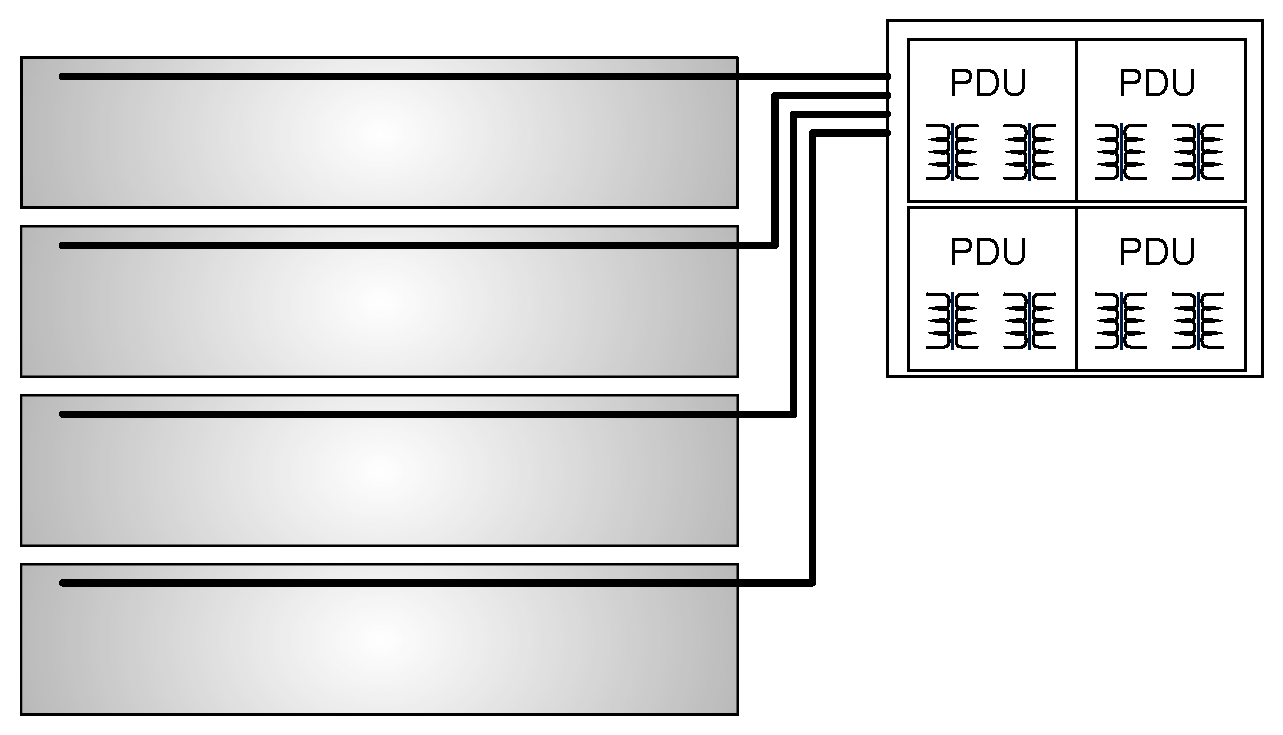
\includegraphics[scale=.3]{Appendices/PowerRouting/figure/full2.eps}
\label{figure::connected}
}
\qquad
\subfigure[Serpentine]{
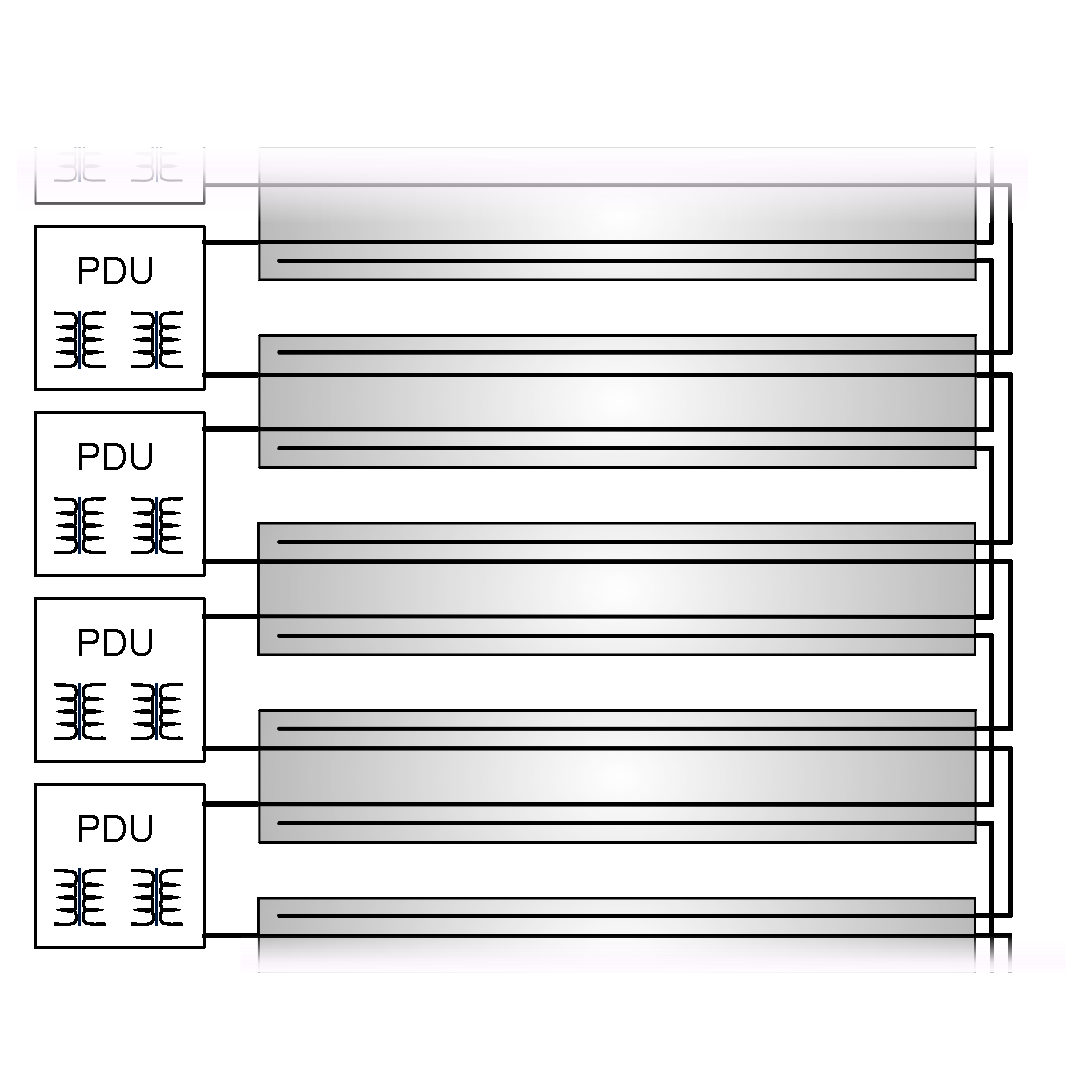
\includegraphics[scale=.3]{Appendices/PowerRouting/figure/ring.eps}
\label{figure::ring}
}
\hspace{0.5in}
\subfigure[X-Y]{
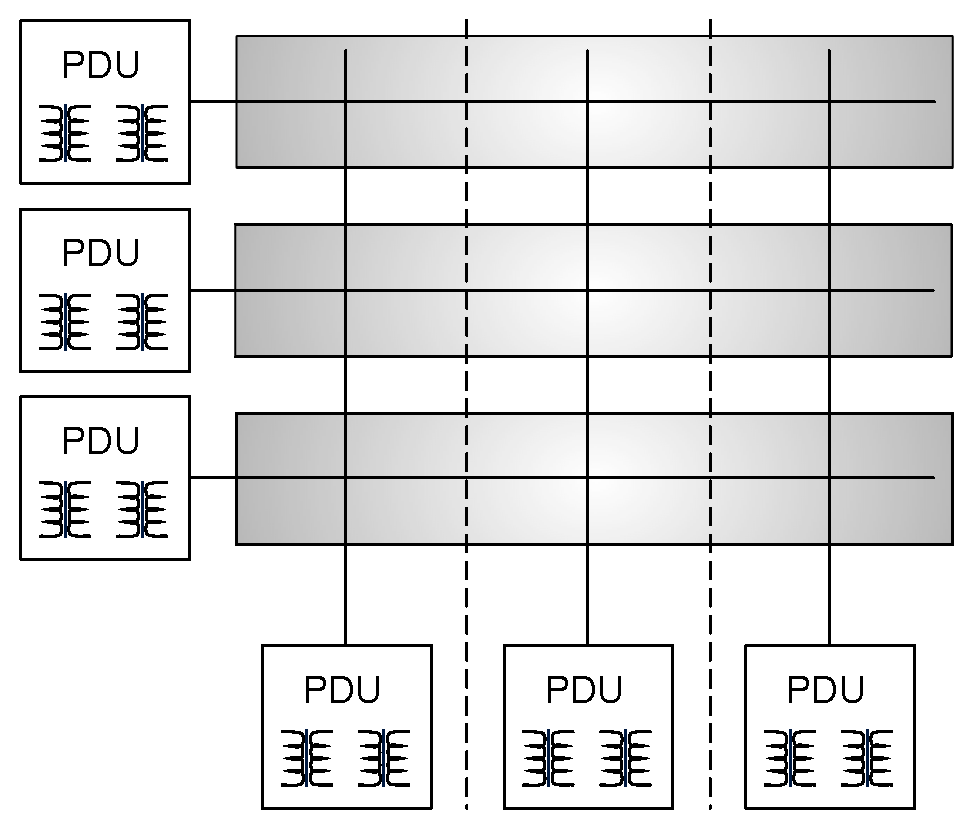
\includegraphics[scale=.3]{Appendices/PowerRouting/figure/xy3.eps}
\label{figure::xy}
}

\vspace{-0.10 in}
\caption{ \textbf{Shuffled power distribution topologies.} }
\vspace{-0.15 in}
\label{figure::topologies}
\end{figure*}

In high-availability data centers, servers are connected to two PDUs to ensure uninterrupted operation in the event of a PDU fault.  A naive (but not unusual) connection topology provisions paired PDUs for each cluster of machines.  Under this data center design, each PDU must be sized to support the full worst-case load of the entire cluster; hence, the power infrastructure is 50\% utilized in the best case. As described in Section~\ref{section::background}, the more sophisticated ``wrapped" topology shown in Figure~\ref{section::background} splits a failed PDU's load over two neighbors, allowing each PDU to be sized to support only 150\% of its nominal primary load.  

By spreading the responsibility for failover further, to additional PDUs, the spare capacity required of each PDU can be reduced---the more PDUs that cooperate to cover the load of a failed PDU, the less reserve capacity is required in the data center as a whole.  In effect, the reserve capacity in each PDU protects multiple loads (which is acceptable provided there is only a single failure). 

Figure~\ref{figure::failover} illustrates the differing reserve capacity requirements of the wrapped topology and a shuffled topology where responsibility for reserve capacity is spread over three PDUs.  The required level of reserve capacity at each PDU is approximately $X / N$, where $X$ represents the cluster power demand, and $N$ the number of PDUs cooperating to provide reserve capacity. (Actual reserve requirements may vary depending on the instantaneous load on each phase).

The savings from shuffled topologies do not require any intelligent switching capability; rather, they require only increased diversity in the distinct combinations of primary and secondary power feeds for each server (ideally covering all combinations equally).   

The layout of PDUs and power busses must be carefully considered to yield feasible shuffled wiring topologies.   Our distribution strategies rely on overhead power busses \cite{Rasmussen129} rather than conventional under-floor conduits to each rack.  The power busses make it easier (and less costly) to connect many, distant racks to a PDU.  Power from each nearby bus is routed to a panel at the top of each rack, and these in turn connect to vertical whips (i.e., outlet strips) that supply power to individual servers.  The whips provide outlets in pairs (or a single outlet with an internal transfer switch) to make it easy to connect servers while assuring an appropriate mix of distinct primary and secondary power feed combinations.

Though overhead power busses are expensive, they still account for a small fraction of the cost of large-scale data center power infrastructure.  Precise quantification of wiring costs is difficult without detailed facility-specific architecture and engineering. We neglect differences in wiring costs when estimating data center infrastructure costs, and instead examine the (far more significant) impact that topologies have on the capacity requirements of the high-voltage infrastructure.  The primary difficulty of complex wiring topologies lies in engineering the facility-specific geometry of the large (and dangerous) high-current overhead power rails; a challenge that we believe is surmountable.

We propose three shuffled power distribution topologies that improve on the wrapped topology of current high-availability data centers.  The \emph{fully connected} topology collocates all PDUs in one corner of the room, and routes power from all PDUs throughout the entire facility.  This topology is not scalable. However, we study it as it represents an upper bound on the benefits of shuffled topologies. We further propose two practical topologies.  The \emph{X-Y} topology divides the data center into a checkerboard pattern of power zones, routing power both north-south and east-west across the zones.  The \emph{serpentine} topology extends the concept of the wrapped topology (see Figure~\ref{figure::redundant}) to create overlap among neighboring PDUs separated by more than one row.

Each distribution topology constrains the set of power feed combinations available in each rack in a different manner.  These constraints in turn affect the set of choices available to the \PowerRouting scheduler, thereby impacting its effectiveness.  


\textbf{Wrapped Topology}.  Figure~\ref{figure::wrapped} illustrates the wrapped topology, which is our term for the conventional  high-availability data center topology (also seen in Figure~\ref{figure::redundant}).  This topology provides limited connectivity to PDUs, and is insufficient for \PowerRouting. 

\textbf{Fully-connected Topology}.  Figure~\ref{figure::connected} illustrates the fully-connected topology.  Under this topology, power is routed from every PDU to every rack. As noted above, the fully-connected topology does not scale and is impractical in all but the smallest data centers.  However, one scalable alternative is to organize the data center as disconnected islands of fully-connected PDUs and rack clusters.  Such a topology drastically limits \PowerRouting flexibility, but can scale to arbitrary-sized facilities.

\textbf{Serpentine Topology}.  Figure~\ref{figure::ring} illustrates the serpentine topology.  Under this topology, PDUs are located at one end of the data centers' rows, as in the wrapped topology shown in Figure~\ref{figure::redundant}.  However, whereas in the wrapped topology a power bus runs between two equipment rows from the PDU to the end of the facility, in the serpentine topology, the power bus then bends back, returning along a second row.  This snaking bus pattern is repeated for each PDU, such that two power busses run in each aisle and four busses are adjacent to each equipment row.  The pattern scales to larger facilities by adding PDUs and replicating the pattern over additional rows.  It scales to higher PDU connectivity by extending the serpentine pattern with an additional turn.

\textbf{X-Y Topology}.  Figure~\ref{figure::xy} illustrates the X-Y topology. Under this topology, the data center is divided into square zones in a checkerboard pattern.  PDUs are located along the north and west walls of the data center.  Power busses from each PDU route either north-south or east-west along the centerline of a row (column) of zones.  Hence, two power busses cross in each zone.  These two busses are connected to each rack in the zone. This topology scales to larger facilities in a straight-forward manner, by adding zones to the ``checkerboard."  It scales to greater connectivity by routing power busses over the zones in pairs (or larger tuples).



\subsection{Power Routing.}

\PowerRouting leverages shuffled topologies to achieve further capital cost savings by under-provisioning PDUs relative to worst-case demand.   The degree of under-provisioning is a business decision made at design time (or when deploying additional systems) based on the probability of utilization spikes and the cost of performance throttling (i.e., the risk of failing to meet a service-level agreement).  \PowerRouting shifts spare capacity to cover local power demand spikes by controlling the assignment of each server to its primary or secondary feed.  The less correlation there is among spikes, the more effective \PowerRouting will be at covering those spikes by shifting loads rather than throttling performance.  \PowerRouting relies on a capping mechanism to prevent overloads when spikes cannot be covered.

\PowerRouting employs a centralized control mechanism to assign each server to its primary or secondary power feed and set power budgets for each server to assure PDU overloads do not occur.  Each time a server's power draw increases to its pre-determined cap (implying that performance throttling will be engaged), the server signals the \PowerRouting controller to request a higher cap.  If no slack is available on the server's currently active power feed, the controller invokes a scheduling algorithm (detailed in Section~\ref{section::scheduling}) to determine new power budgets and power feed assignments for all servers to try to locate slack elsewhere in the power distribution system.  The controller will reduce budgets for servers whose utilization has decreased and may reassign servers between their primary and secondary feeds to create the necessary slack.  If no solution can be found (e.g., because aggregate power demand exceeds the facilities' total provisioning), the existing power cap remains in place and the server's performance is throttled.  

In addition to trying to satisfy each server's desired power budget, the \PowerRouting scheduler also maintains sufficient reserve capacity at each PDU to ensure continued operation (under the currently-established power budgets) even if any single PDU fails.  A PDU's required reserve capacity is given by the largest aggregate load served by another PDU for which it acts as the secondary (inactive) feed.

Finally, the \PowerRouting scheduler seeks to balance load across the three AC phases of each PDU.  As noted in Section~\ref{section::background}, phase imbalance can lead to numerous electrical problems that impact safety and availability.  The scheduler constrains the current on each of the three phases to remain within a 20\% margin.

The key novelty of \PowerRouting lies in the assignment of servers to power feeds; sophisticated budgeting mechanisms (e.g., which assign asymmetric budgets to achieve higher-level QoS goals) have been extensively studied \cite{Ranganathan06,Lefurgy08,Wang08, Femal05,Raghavendra08,Wang09,Nathuji07,Gandhi09b}.  Hence, in this paper, we focus our design and evaluation on the power feed scheduling mechanism and do not explore QoS-aware capping in detail.

\subsection{Implementation.}

\PowerRouting comprises four elements: (1) an actuation mechanism to switch servers between their two redundant power feeds; (2) the centralized controller that executes the power feed scheduling algorithm;  (3) a communications mechanism for the controller to direct switching activity and assign budgets; and (4) a power distribution topology that provisions primary and secondary power feeds in varying combinations to the receptacles in each rack.   

\textbf{Switching power feeds}. The power feed switching mechanism differs for single- and dual-corded servers.  In a single-corded server, an external transfer switch attaches the server to its primary or secondary power feed.  In the event of a power interruption on the active feed, the transfer switch seamlessly switches the load to the alternative feed (a local, automatic action).  The scheduler assures that all PDUs have sufficient reserve capacity to supply all loads that may switch to them in the event of any single PDU failure.  To support phase balancing, the transfer switch must be capable of switching loads across out-of-phase AC sources fast enough to appear uninterrupted to computer power supplies.  External transfer switches of this sort are in wide-spread use today, and retail for several hundred dollars. In contrast to existing transfer switches, which typically switch entire circuits (several servers), \PowerRouting requires switching at the granularity of individual receptacles, implying somewhat higher cost. For dual-corded servers, switching does not require any additional hardware, as the switching can be accomplished through the systems' internal power supplies. 

\textbf{Control unit}. The \PowerRouting control unit is a microprocessor that orchestrates the power provisioning process.  Each time scheduling is invoked, the control unit performs four steps: (1) it determines the desired power budget for each server; (2) it schedules each server to its primary or secondary power feed; (3) it assigns a power cap to each server (which may be above the request, allowing headroom for utilization increase, or below, implying performance throttling); and (4) it communicates the power cap and power feed assignments to all devices.  The control unit can be physically located within the existing intelligence units in the power delivery infrastructure (most devices already contain sophisticated, network-attached intelligence units). Like other power system components, the control unit must include mechanisms for redundancy and fault tolerance.  Details of the control unit's hardware/software fault tolerance are beyond the scope of this study; the challenges here mirror those of the existing intelligence units in the power infrastructure.  

The mechanisms used in each of the control unit's four steps are orthogonal. As this study is focused on the novel scheduling aspect of \PowerRouting (step 2), we explore only relatively simplistic policies for the other steps.  We determine each server's desired power budget based in its peak demand in the preceding minute.  Our power capping mechanism assigns power budgets that throttle servers to minimize the total throttled power.
%\fixme{Add a comment citing work with more intelligent capping policies.}

\textbf{Communication.} Communication between the control unit and individual servers/transfer switches is best accomplished over the data center's existing network infrastructure, for example, using the Simple Network Management Protocol (SNMP) or BACnet.  The vast majority of power provisioning infrastructure already supports these interfaces.  Instantaneous server power draws and power budgets can also typically be accessed through SNMP communication with the server's Integrated Lights Out (ILO) interface. 

\textbf{Handling uncontrollable equipment.} Data centers contain myriad equipment that draw power, but cannot be controlled by \PowerRouting (e.g., network switches, monitors).  The scheduler must account for the worst-case power draw of such equipment when calculating available capacity on each PDU and phase.

\begin{figure}[b]
\centering
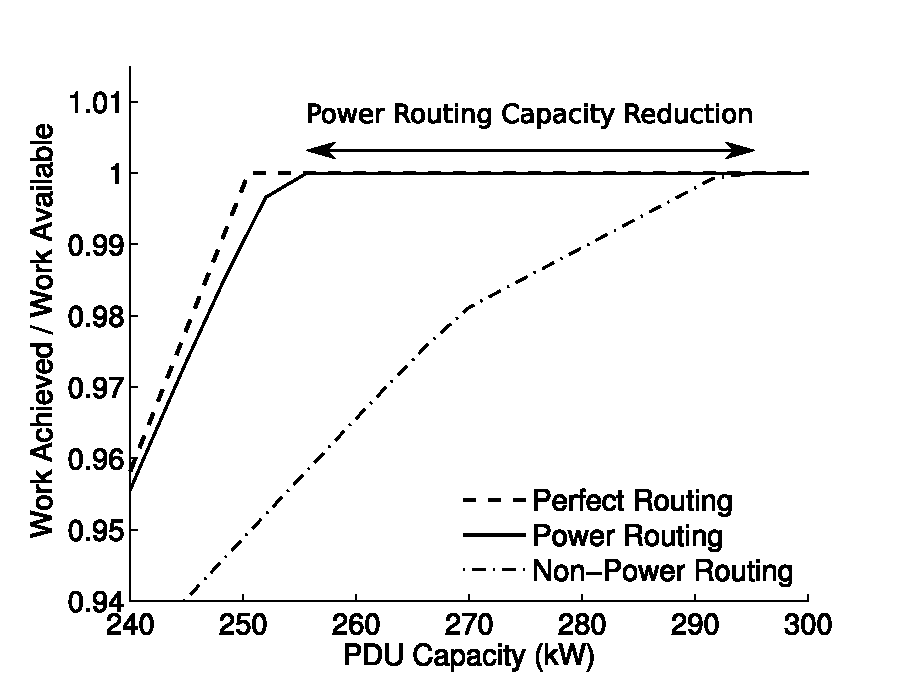
\includegraphics[width = 3.0 in]{Appendices/PowerRouting/figure/RoutingComparison.eps}
\caption{ \textbf{Shuffled Topologies: 6 PDUs, fully-connected}}
\label{figure::routingdemonstration}
\vspace{-.1 in}
\end{figure}

\subsection{Operating Principle.}

\PowerRouting relies on the observation that individual PDUs are unlikely to reach peak load simultaneously.
The power distribution system as a whole operates in one of three regimes.
The first, most common case is that the load on all PDUs is below their capacity.  In this case, the power infrastructure is over-provisioned, power capping is unnecessary, and the entire data center operates at full performance. At the opposite extreme, when servers demand more power than is available, the power infrastructure is under-provisioned, all PDUs will be fully loaded, and power capping (e.g., via performance throttling) is necessary.  In either of these regimes, \PowerRouting has no impact; the power infrastructure is simply under- (over-) provisioned relative to the server demand. 

\PowerRouting is effective in the intermediate regime where some PDUs are overloaded while others have spare capacity.  In current data centers, this situation will result in performance throttling that \PowerRouting can avoid.

To illustrate how \PowerRouting affects performance throttling, we explore its performance envelope near the operating region where aggregate power infrastructure capacity precisely meets demand.  Figure~\ref{figure::routingdemonstration} shows the relationship between installed PDU capacity and performance throttling (in terms of the fraction of offered load that is met) with and without  \PowerRouting (6 PDUs, fully-connected topology) and contrast these against an ideal, perfectly-balanced power distribution infrastructure.    The ideal infrastructure can route power from any PDU to any server and can split load fractionally over multiple PDUs.  (We detail the methodology used to evaluate \PowerRouting and produce these results in Section~\ref{section::methodology} below.)

The graph provides two insights into the impact of \PowerRouting.  First, we can use it to determine how much more performance \PowerRouting achieves for a given infrastructure investment relative to conventional and ideal designs.  This result can be obtained by comparing vertically across the three lines for a selected PDU capacity. As can be seen, \PowerRouting closely tracks the performance of the ideal power delivery infrastructure, recovering several percent of lost performance relative to a fully-connected topology without power routing.

The graph can also be used to determine the capital infrastructure savings that \PowerRouting enables while avoiding performance throttling altogether.  Performance throttling becomes necessary at the PDU capacity where each of the three power distributions dips below 1.0.  The horizontal distance between these intercepts is the capacity savings, and is labeled  ``Power Routing Capacity Reduction" in the figure. In the case shown here, \PowerRouting avoids throttling at a capacity of 255 kW, while 294 kW of capacity are needed without \PowerRouting. \PowerRouting avoids throttling, allowing maximum performance with less investment in power infrastructure.
